\subsection{21. Nonparametric Curve Estimation}\label{nonparametric-curve-estimation}

In this Chapter we discuss the nonparametric estimation of probability
density functions and regression functions, which we refer to a
\textbf{curve estimation}.

In Chapter 8 we saw it is possible to consistently estimate a cumulative
distribution function \(F\) without making any assumptions about \(F\).
If we want to estimate a probability density function \(f(x)\) or a
regression function \(r(x) = \mathbb{E}(Y | X = x)\) the situation is
different. We cannot estimate these functions consistently without
making some smoothness assumptions. Correspondingly, we will perform
some sort of smoothing operation with the data.

A simple example of a density estimator is a \textbf{histogram}. To form
a histogram estimator of a density \(f\), we divide the real line into
disjoint sets called \textbf{bins}. The histogram estimator is a
piecewise constant function where the height of the function is
proportional to the number of observations in each bin. The number of
bins is an example of a \textbf{smoothing parameter}. If we smooth too
much (large bins) we get a highly biased estimator while if smooth too
little (small bins) we get a highly variable estimator. Much of curve
estimation is concerned with trying to optimally balance variance and
bias.

\subsubsection{21.1 The Bias-Variance Tradeoff}\label{the-bias-variance-tradeoff}

Let \(g\) denote an unknown function and let \(\hat{g}_n\) denote an
estimator of \(g\). Bear in mind that \(\hat{g}_n(x)\) is a random
function evaluated at a point \(x\); \(\hat{g}_n\) is random because it
depends on the data. Indeed, we could be more explicit and write
\(\hat{g}_n(x) = h_x(X_1, \dots, X_n)\) to show that \(\hat{g}_n(x)\) is
a function of the data \(X_1, \dots, X_n\) and that the function could
be different for each \(x\).

As a loss function, we will use the \textbf{integrated square error
(ISE)}:

\[ L(g, \hat{g}_n) = \int (g(u) - \hat{g}_n(u))^2 du\]

The \textbf{risk} or \textbf{mean integrated square error (MISE)} is:

\[ R(g, \hat{g}) = \mathbb{E}\left(L(g, \hat{g}) \right) \]

\textbf{Lemma 21.1}. The risk can be written as

\[ R(g, \hat{g}) = \int b^2(x) dx + \int v(x) dx \]

where

\[ b(x) = \mathbb{E}(\hat{g}_n(x)) - g(x) \]

is the bias of \(\hat{g}_n(x)\) at a fixed \(x\) and

\[ v(x) = \mathbb{V}(\hat{g}_n(x)) = \mathbb{E}\left( \hat{g}_n(x) - \mathbb{E}(\hat{g}_n(x))^2\right) \]

is the variance of \(\hat{g}_n(x)\) at a fixed \(x\).

In summary,

\[ \text{RISK} = \text{BIAS}^2 + \text{VARIANCE} \]

When the data is over-smoothed, the bias term is large and the variance
is small. When the data are under-smoothed the opposite is true. This is
called the \textbf{bias-variance trade-off}. Minimizing risk corresponds
to balancing bias and variance.

\subsubsection{21.2 Histograms}\label{histograms}

Let \(X_1, \dots, X_n\) be IID on \([0, 1]\) with density \(f\). The
restriction on \([0, 1]\)is not crucial; we can always rescale the data
to be on this interval. Let \(m\) be an integer and define bins

\[ B_1 = \left[0, \frac{1}{m} \right), B_2 = \left[\frac{1}{m}, \frac{2}{m} \right), \dots, B_m = \left[\frac{m - 1}{m}, 1 \right] \]

Define the \textbf{binwidth} \(h = 1 / m\), let \(v_j\) be the number of
observations in \(B_j\), let \(\hat{p}_j = v_j / n\) and let
\(p_j = \int_{B_j} f(u) du\).

The \textbf{histogram estimator} is defined by

\[
\hat{f}_n(x) = \begin{cases}
\hat{p}_1 / h & x \in B_1 \\
\hat{p}_2 / h & x \in B_2 \\
\vdots & \vdots\\
\hat{p}_m / h & x \in B_m
\end{cases}
\]

which we can write more succinctly as

\[ \hat{f}_n(x) = \sum_{j=1}^n \frac{\hat{p}_j}{h} I(x \in B_j) \]

To understand the motivation for this estimator, let
\(p_j = \int_{B_j} f(u) du\) and note that, for \(x \in B_j\) and \(h\)
small,

\[ \hat{f}_n(x) = \frac{\hat{p}_j}{h} \approx \frac{p_j}{h} = \frac{\int_{B_j} f(u) du}{h} \approx \frac{f(x) h}{h} = f(x) \]

The mean and the variance of \(\hat{f}_n(x)\) are given in the following
Theorem.

\textbf{Theorem 21.3}. Consider fixed \(x\) and fixed \(m\), and let
\(B_j\) be the bin containing \(x\). Then,

\[ 
\mathbb{E}(\hat{f}_n(x)) = \frac{p_j}{h} 
\quad \text{and} \quad
\mathbb{V}(\hat{f}_n(x)) = \frac{p_j (1 - p_j)}{nh^2}
\]

Let's take a closer look at the bias-variance tradeoff. Consider some
\(x \in B_j\). For any other \(u \in B_j\),

\[ f(u) \approx f(x) + (u - x) f'(x) \]

and so

\[ 
\begin{align}
p_j = \int_{B_j} f(u) du &\approx \int_{B_j} (f(x) + (u - x) f'(x)) du \\
&= f(x) h + h f'(x) \left(h \left(j - \frac{1}{2} \right) - x \right)
\end{align}
\]

Therefore, the bias \(b(x)\) is

\[
\begin{align}
b(x) &= \mathbb{E}(\hat{f}_n(x)) - f(x) = \frac{p_j}{h} - f(x) \\
&\approx \frac{f(x) h + h f'(x) \left(h \left(j - \frac{1}{2} \right) - x \right)}{h} - f(x) \\
&= f'(x) \left(h \left(j - \frac{1}{2} \right) - x \right)
\end{align}
\]

If \(\overline{x}_j\) is the center of the bin, then

\[
\begin{align}
\int_{B_j} b^2(x) dx &= \int_{B_j} (f'(x))^2 \left(h \left(j - \frac{1}{2} \right) - x \right)^2 dx \\
&\approx (f'(\overline{x}_j))^2 \int_{B_j} \left(h \left(j - \frac{1}{2} \right) - x \right)^2 dx \\
&= (f'(\overline{x}_j))^2 \frac{h^3}{12}
\end{align}
\]

Therefore,

\[
\begin{align}
\int_0^1 b^2(x) dx &= \sum_{j=1}^m \int_{B_j} b^2(x) dx \approx \sum_{j=1}^m (f'(\overline{x}_j))^2 \frac{h^3}{12} \\
&= \frac{h^2}{12} \sum_{j=1}^m h(f'(\overline{x}_j))^2 \approx \frac{h^2}{12} \int_0^1 h(f'(\overline{x}_j))^2 dx
\end{align}
\]

Note that this increases as a function of \(h\).

Now consider the variance. For \(h\) small, \(1 - p_j \approx 1\), so

\[
\begin{align}
v(x) &\approx \frac{p_j}{nh^2}\\
&= \frac{f(x)h + h f'(x)\left(h \left(j - \frac{1}{2} \right) - x \right)}{nh^2} \\
&\approx \frac{f(x)}{nh}
\end{align}
\]

when we keep the dominant term. So

\[
\int_0^1 v(x) dx \approx \frac{1}{nh}
\]

Note that this decreases with \(h\). Putting this all together, we get:

\textbf{Theorem 21.4}. Suppose that \(\int (f'(u))^2 du < \infty\). Then

\[ R(\hat{f}_n, f) \approx \frac{h^2}{12} \int (f'(u))^2 du + \frac{1}{nh}\]

The value \(h^*\) that minimizes this expression is

\[ h^* = \frac{1}{n^{1/3}} \left( \frac{6}{\int (f'(u))^2 du} \right)^{1/3}\]

With this choice of binwidth,

\[ R(\hat{f}_n, f) \approx \frac{C}{n^{2/3}} \]

where \(C = (3/4)^{2/3} \left( \int (f'(u))^2 du \right)^{1/3}\).

Theorem 21.4 is quite revealing. We see that with an optimally chosen
bandwidth, the MISE decreases to 0 at rate \(n^{-2/3}\). By comparison,
most parametric estimators converge at rate \(n^{-1}\). The formula for
optimal binwidth \(h^*\) is of theoretical interest but it is not useful
in practice since it depends on the unknown function \(f\).

A practical way of choosing the binwidth is to estimate the risk
function and minimize over \(h\). Recall that the loss function, which
we now write as a function of \(h\), is

\[
\begin{align}
L(h) &= \int \left( \hat{f}_n(x) - f(x) \right)^2 dx \\
&= \int \hat{f}_n^2(x) dx - 2 \int \hat{f}_n(x) f(x) dx + \int f^2(x) dx
\end{align}
\]

The last term does not depend on the binwidth \(h\) so minimizing the
risk is equivalent to minimizing the expected value of

\[ J(h) = \int \hat{f}_n^2(x) dx - 2 \int \hat{f}_n(x) f(x) dx \]

We shall refer to \(\mathbb{E}(J(h))\) as the risk, although it differs
from the true risk by the constant term \(\int f^2(x) dx\).

The \textbf{cross-validation estimator of risk} is

\[ \hat{J}(h) = \int \left( \hat{f}_n(x) \right)^2 dx - \frac{2}{n} \sum_{i=1}^n \hat{f}_{(-i)}(X_i)\]

where \(\hat{f}_{(-i)}\) is the histogram estimator obtained after
removing the \(i\)-th observation. We refer to \(\hat{J}(h)\) as the
cross-validation score or estimated risk.

\textbf{Theorem 21.6}. The cross-validation estimator is nearly
unbiased:

\[ \mathbb{E}(\hat{J}(x)) \approx \mathbb{E}(J(x)) \]

In principle, we need to recompute the histogram \(n\) times to compute
\(\hat{J}(x)\). Moreover, this has to be done for all values of \(h\).
Fortunately, there is a shortcut formula.

\textbf{Theorem 21.7}. The following identity holds:

\[ \hat{J}(h) = \frac{2}{(n - 1)h} + \frac{n+1}{n-1} \sum_{j=1}^m \hat{p}_j^2 \]

Next we want some sort of confidence set for \(f\). Suppose
\(\hat{f}_n\) is a histogram with \(m\) bins and binwidth \(h = 1 / m\).
We cannot realistically make confidence statements about the fine
details of true density \(f\). Instead, we make confidence statements
about \(f\) at the resolution of the histogram. To this end, define

\[ \overline{f}(x) = \frac{p_j}{h} \quad \text{for } x \in B_j \]

where \(p_j = \int_{B_j} f(u) du\) which is a ``histogramized'' version
of \(f\).

\textbf{Theorem 21.9}. Let \(m = m(n)\) be the number of bins in the
histogram \(\hat{f}_n\). Assume that \(m(n) \rightarrow \infty\) and
\(m(n) \log m / n \rightarrow 0\) as \(n \rightarrow \infty\). Define

\[
\ell(x) = \left( \text{max} \left\{\sqrt{\hat{f}_n(x)} - c, 0\right\} \right)^2
\quad \text{and} \quad
u(x) = \left(\sqrt{\hat{f}_n(x)} + c \right)^2
\]

where

\[
c = \frac{z_{\alpha / (2 m)}}{2} \sqrt{\frac{m}{n}}
\]

Then,

\[
\lim_{n \rightarrow \infty} \mathbb{P} \left( \ell(x) \leq \overline{f}(x) \leq u(x) \text{ for all } x \right) \geq 1 - \alpha
\]

\textbf{Proof}. Here is an outline of the proof. A rigorous proof
requires fairly sophisticated tools. From the central limit theorem,
\(\hat{p}_j \approx N\left(p_j, p_j (1 - p_j) / n\right)\). By the delta
method, \(\sqrt{\hat{p}_j} \approx N\left(\sqrt{p_j}, 1 / (4n)\right)\).
Moreover, it can be shown that the \(\sqrt{\hat{p}_j}\)'s are
approximately independent. Therefore,

\[ 2 \sqrt{n} \left( \sqrt{\hat{p}_j} - \sqrt{p_j} \right) \approx Z_j \]

where \(Z_1, \dots, Z_m \sim N(0, 1)\). Let \(A\) be the event that
\(\ell(x) \leq \overline{f}(x) \leq u(x)\) for all \(x\). So,

\[
\begin{align}
A &= \left\{ \ell(x) \leq \overline{f}(x) \leq u(x) \text{ for all } x \right\} \\
&= \left\{ \sqrt{\ell(x)} \leq \sqrt{\overline{f}(x)} \leq \sqrt{u(x)} \text{ for all } x \right\} \\
&= \left\{ \sqrt{\hat{f}_n(x)} - c \leq \sqrt{\overline{f}(x)} \leq \sqrt{\hat{f}_n(x)} + c \text{ for all } x \right\} \\
&= \left\{ \max_x \left| \sqrt{\hat{f}_n(x)} - \sqrt{\overline{f}(x)} \right| \leq c \right\}
\end{align}
\]

Therefore,

\[
\begin{align}
\mathbb{P}(A^c) &= \mathbb{P} \left( \max_x \left| \sqrt{\hat{f}_n(x)} - \sqrt{\overline{f}(x)} \right| > c\right)
= \mathbb{P} \left( \max_j \left| \sqrt{\frac{\hat{p}_j}{h}} - \sqrt{\frac{p_j}{h}} \right| > c\right) \\
&= \mathbb{P} \left( \max_j \left| \sqrt{\hat{p}_j} - \sqrt{p_j} \right| > c \sqrt{h} \right)
= \mathbb{P} \left( \max_j 2 \sqrt{n} \left| \sqrt{\hat{p}_j} - \sqrt{p_j} \right| > 2 c \sqrt{hn} \right) \\
&= \mathbb{P} \left( \max_j 2 \sqrt{n} \left| \sqrt{\hat{p}_j} - \sqrt{p_j} \right| > z_{\alpha / (2m)} \right) \\
&\approx \mathbb{P} \left( \max_j \left| Z_j \right| > z_{\alpha / (2m)} \right)
 \leq \sum_{j=1}^m \mathbb{P} \left( \max_j \left| Z_j \right| > z_{\alpha / (2m)} \right) \\
&= \sum_{j=1}^m \frac{\alpha}{m} = \alpha
\end{align}
\]

\subsubsection{21.3 Kernel Density Estimation}\label{kernel-density-estimation}

Histograms are discontinuous. \textbf{Kernel density estimators} are
smoother and they converge faster to the true density than histograms.

Let \(X_1, \dots, X_n\) denote the observed data, a sample from \(f\).
In this chapter, a \textbf{kernel} is defined to be any smooth function
\(K\) such that \(K(x) \geq 0\), \(\int K(x) dx = 1\),
\(\int x K(x) dx = 0\) and \(\sigma_K^2 \equiv \int x^2 K(x) dx > 0\).
Two examples of kernels are the \textbf{Epanechnikov kernel}

\[ K(x) = \begin{cases}
\frac{3}{4} \left(1 - x^2 / 5 \right) / \sqrt{5} & \text{if } |x| < \sqrt{5} \\
0 & \text{otherwise}
\end{cases}\]

and the Gaussian (Normal) kernel \(K(x) = (2\pi)^{-1/2} e^{-x^2/2}\).

Given a kernel \(K\) and a positive number \(h\), called the
\textbf{bandwidth}, the \textbf{kernel density estimator} is defined to
be

\[ \hat{f}(x) = \frac{1}{n} \sum_{i=1}^n \frac{1}{h} K \left( \frac{x - X_i}{h} \right) \]

The kernel density estimator effectively puts a smoothed out lump of
mass \(1 / n\) over each data point \(X_i\). The bandwidth \(h\)
controls the amount of smoothing. When \(h\) is close to 0,
\(\hat{f}_n\) consists of a set of spikes, one at each data point. The
height of the spikes tends to infinity as \(h \rightarrow 0\). When
\(h \rightarrow 0\), \(\hat{f}_n\) tends to a uniform density.

To construct a kernel density estimator, we need to choose a kernel
\(K\) and a bandwidth \(h\). It can be shown theoretically and
empirically that the choice of \(K\) is not crucial. However, the choice
of bandwidth \(h\) is very important. As with the histogram, we can make
a theoretical statement about how the risk of the estimator depends on
the bandwidth.

\textbf{Theorem 21.13}. Under weak assumptions on \(f\) and \(K\),

\[ R(f, \hat{f}_n) \approx \frac{1}{4} \sigma_K^4 h^4 \int \left(f''(x)\right)^2 dx + \frac{\int K^2(x) dx}{nh} \]

where \(\sigma_K^2 = \int x^2 K(x) dx\). The optimal bandwidth is

\[ h^* = \frac{c_1^{-2/5} c_2^{1/5} c_3^{-1/5}}{n^{1/5}} \]

where \(c_1 = \int x^2 K(x) dx\), \(c_2 = \int K(x)^2 dx\) and
\(c_3 = \int \left( f''(x) \right)^2 dx\). With this choice of
bandwidth,

\[ R(f, \hat{f}_n) \approx \frac{c_4}{n^{4/5}} \]

for some constant \(c_4 > 0\).

\textbf{Proof}. Let

\[ K_h(x, X) = \frac{1}{h} K\left( \frac{x - X}{h} \right)
\quad \text{and} \quad
\hat{f}_n(x) = \frac{1}{n} \sum_{i=1}^n K_h(x, X_i)
\]

Thus, \[
\begin{align}
\mathbb{E}[\hat{f}_n(x)] &= \mathbb{E}[K_h(x, X)] \\
\mathbb{V}[\hat{f}_n(x)] &= \frac{1}{n} \mathbb{V}[K_h(x, X)]
\end{align}
\]

Now,

\[
\begin{align}
\mathbb{E}[K_h(x, X)] &= \int \frac{1}{h} K\left( \frac{x - t}{h} \right) f(t) dt \\
&= \int K(u) f(x - hu) du \\
&= \int K(u) \left[ f(x) - hu f'(x) + \frac{1}{2} h^2u^2 f''(x) + \dots \right] du \\
&= f(x) + \frac{1}{2} h^2 f''(x) \int u^2 K(u) du + \dots
\end{align}
\]

since \(\int K(u) du = 1\) and \(\int u K(u) du = 0\). The bias is

\[ \mathbb{E}[K_h(x, X)] - f(x) \approx \frac{1}{2} \sigma_K^2 h^2 f''(x) \]

By a similar calculation,

\[ \mathbb{V}[\hat{f}_n(x)] \approx \frac{f(x) \int K^2(u) du}{n h_n} \]

The second result follows from integrating the bias squared plus
variance.

We see that kernel estimators converge at rate \(n^{-4/5}\) while
histograms converge at rate \(n^{-2/3}\). It can be shown that, under
weak assumptions, there does not exist a nonparametric estimator that
converges faster than \(n^{-4/5}\).

The expression for \(h^*\) depends on the unknown density \(f\) which
makes the result of little practical use. As with the histograms, we
shall use cross-validation to find a bandwidth. Thus, we estimate the
risk (up to a constant) by

\[ \hat{J}(h) = \int \hat{f}^2(x) dx - 2 \frac{1}{n} \sum_{i=1}^n \hat{f}_{-i}(X_i) \]

where \(\hat{f}_{-i}\) is the kernel density estimator after omitting
the \(i\)-th observation.

\textbf{Theorem 21.14}. For any \(h > 0\),

\[ \mathbb{E} \left[ \hat{J}(h) \right] = \mathbb{E} \left[ J(h) \right] \]

Also,

\[ \hat{J}(h) \approx \frac{1}{hn^2}\sum_{i, j} K^* \left( \frac{X_i - X_j}{h} \right) + \frac{2}{nh} K(0) \]

where \(K^*(x) = K^{(2)}(x) - 2 K(x)\) and
\(K^{(2)}(z) = \int K(z - y) K(y) dy\). In particular, if \(K\) is a
\(N(0, 1)\) Gaussian kernel then \(K^{(2)}(z)\) is the \(N(0, 2)\)
density.

We then choose the bandwidth \(h_n\) that maximizes \(\hat{J}(h)\). A
justification for this method is given by the following remarkable
theorem due to Stone.

\textbf{Theorem 21.15 (Stone's Theorem)}. Suppose that \(f\) is bounded.
Let \(\hat{f}_h\) denote the kernel estimator with bandwidth \(h\) and
let \(h_n\) denote the bandwidth chosen by cross-validation. Then,

\[ \frac{\int \left( f(x) - \hat{f}_{h_n}(x)\right)^2 dx}{\inf_h \int \left( f(x) - \hat{f}_h(x) \right)^2 dx} \xrightarrow{\text{P}} 1\]

To construct confidence bands, we use something similar to histograms
although the details are more complicated. The version described here is
from Chaudhuri and Marron (1999).

\textbf{Confidence Band for Kernel Density Estimator}

\begin{enumerate}[tightlist,label={\arabic*.}]
\item
  Choose an evenly spaced grid of points
  \(\mathcal{V} = \{ v_1, \dots, v_N \}\). For every
  \(v \in \mathcal{V}\), define
\end{enumerate}

\[ Y_i(v) = \frac{1}{h} K \left( \frac{v - X_i}{h} \right) \]

Note that \(\hat{f}_n(v) = \overline{Y}_n(v)\), the average of the
\(Y_i(v)\)'s.

\begin{enumerate}[tightlist,label={\arabic*.}]
\item
  Define
\end{enumerate}

\[ \text{se}(v) = \frac{s(v)}{\sqrt{n}} \]

where
\(s^2(v) = (n - 1)^{-1} \sum_{i=1}^n ( Y_i(v) - \overline{Y}_n(v) )^2\).

\begin{enumerate}[tightlist,label={\arabic*.},resume]
\item
  Compute the effective sample size
\end{enumerate}

\[ \text{ESS}(v) = \frac{\sum_{i=1}^n K\left( \frac{v - X_i}{h} \right)}{K(0)} \]

\begin{enumerate}[tightlist,label={\arabic*.},resume]
\item
  Let
  \(\mathcal{V}^* = \left\{ v \in \mathcal{V} : \text{ESS}(v) \geq 5 \right\}\).
  Now define the number of independent blocks \(m\) by
\end{enumerate}

\[ \frac{1}{m} = \frac{\overline{\text{ESS}}}{n} \]

where \(\overline{\text{ESS}}\) is the average of \(\text{ESS}\) over
\(\mathcal{V}^*\).

\begin{enumerate}[tightlist,label={\arabic*.},resume]
\item
  Let
\end{enumerate}

\[ q = \Phi^{-1} \left( \frac{1 + (1 + \alpha)^{1/m}}{2} \right) \]

and define

\[ \ell(v) = \text{max} \left\{ \hat{f}_n(v) - q \cdot \text{se}(v), 0 \right\}
\quad \text{and} \quad
u(v) = \hat{f}_n(v) + q \cdot \text{se}(v)\]

Then,

\[ \mathbb{P} \Big\{ \ell(v) \leq f(v) \leq u(v) \text{ for all } v \Big\} \approx 1 - \alpha \]

Suppose now that the data \(X_i = \{ X_{i1}, \dots, X_{id} \}\) are
\(d\)-dimensional. The kernel estimator can easily be generalized to
\(d\) dimensions. Let \(h = (h_1, \dots, h_d)\) be a vector of
bandwidths and define

\[ \hat{f}_n(x) = \frac{1}{n} \sum_{i=1}^n K_h(x - X_i) \]

where

\[ K_h(x - X_i) = \frac{1}{n \prod_{j=1}^d h_j} \left\{ \prod_{j=1}^d K \left( \frac{x_i - X_{ij}}{h_j} \right) \right\} \]

For simplicity, we might take \(h_j = s_j h\) where \(s_j\) is the
standard deviation of the \(j\)-th variable. There is now only a single
bandwidth to choose. Using calculations like the ones in the
one-dimensional case, the risk is given by

\[
R(f, \hat{f}_n) 
\approx \frac{1}{4} \sigma_K^4 \left[ \sum_{j=1}^d h_j^4 \int f_{jj}^2(x) dx + \sum_{j \neq k} h_j^2 h_k^2 \int f_{jj}(x) f_{kk}(x) dx \right] + \frac{\left( \int K^2(x) dx\right)^d}{n \prod_{j=1}^d h_j}
\]

where \(f_{jj}\) is the second partial derivative of \(f\).

The optimal bandwidth satisfies \(h_i \approx c_1 n^{-1/(4 + d)}\)
leading to a risk of order \(n^{-4/(4+d)}\). From this fact, we see that
the risk increases quickly with dimension, a problem usually called the
\textbf{curse of dimensionality}. To get a sense of how serious this
problem is, consider the following table from Silverman (1986) which
shows the sample size required to ensure a relative mean squared error
less than 0.1 at 0 when the density is a multivariate normal and the
optimal bandwidth is selected.

\begin{longtable}[]{@{}ll@{}}
\toprule
Dimension & Sample Size \\
\midrule
\endhead
1 & 4 \\
2 & 19 \\
3 & 67 \\
4 & 223 \\
5 & 768 \\
6 & 2790 \\
7 & 10700 \\
8 & 43700 \\
9 & 187000 \\
10 & 842000 \\
\bottomrule
\end{longtable}

This is bad news indeed. it says that having 842,000 observations in a
ten dimensional problem is really like having 4 observations.

\subsubsection{21.4 Nonparametric Regression}\label{nonparametric-regression}

Consider pairs of points \((x_1, Y_1), \dots, (x_n, Y_n)\) related by

\[ Y_i = r(x_i) + \epsilon_i \]

where \(\mathbb{E}(\epsilon_i) = 0\) and we are treating the \(x_i\)'s
as fixed. In nonparametric regression, we want to estimate the
regression function \(r(x) = \mathbb{E}(Y | X = x)\).

There are many nonparametric regression estimators. Most involve
estimating \(r(x)\) by taking some sort of weighted average of the
\(Y_i\)'s, giving higher weight to those points near \(x\). In
particular, the \textbf{Nadaraya-Watson kernel estimator} is defined by

\[ \hat{r}(x) = \sum_{i=1}^n w_i(x) Y_i\]

where the weights \(w_i(x)\) are given by

\[ w_i(x) = \frac{K\left(\frac{x - x_i}{h}\right)}{\sum_{j=1}^n \left(\frac{x - x_j}{h}\right) } \]

The form of this estimators comes from first estimating the joint
density \(f(x, y)\) using kernel density estimation and then inserting
this into:

\[ r(x) = \mathbb{E}(Y | X = x) = \int y f(y | x) dy = \frac{\int y f(x, y) dy}{\int f(x, y) dy} \]

\textbf{Theorem 21.19}. Suppose that
\(\mathbb{V}(\epsilon_i) = \sigma^2\). The risk of the Nadaraya-Watson
kernel estimator is

\[ R(\hat{r}_n, r) \approx \frac{h^4}{4} 
\left( \int x^2 K^2(x) dx\right)^4
\int \left( r''(x) + 2 r'(x) \frac{f'(x)}{f(x)} \right)^2 dx
+ \int \frac{\sigma^2 \int K^2(x) dx}{nh f(x)} dx
\]

The optimal bandwidth decreases at rate \(n^{-1/5}\) and with this
choice the risk decreases at rate \(n^{-4/5}\).

In practice, to choose the bandwidth \(h\) we minimize the
cross-validation score

\[ \hat{J}(h) = \sum_{i=1}^n (Y_i - \hat{r}_{-i}(x_i))^2\]

where \(\hat{r}_{-i}\) is the estimator we get by omitting the \(i\)-th
variable. An approximation to \(\hat{J}\) is given by

\[ \hat{J}(h) \approx \sum_{i=1}^n (Y_i - \hat{r}(x_i))^2 \left( 1 - \frac{K(0)}{\sum_{j=1}^n K \left( \frac{x_i - x_j}{h} \right)} \right)^{-2}\]

The procedure for finding confidence bands is similar to that for
density estimation. However, we first need to estimate \(\sigma^2\).
Suppose that the \(x_i\)'s are ordered. Assuming \(r(x)\) is smooth, we
have \(r(x_{i+1}) - r(x) \approx 0\) and hence

\[Y_{i+1} - Y_i = \left[ r(x_{i+1} + \epsilon_{i+1} \right] - \left[ r(x_{i} + \epsilon_{i} \right] \approx \epsilon_{i+1} - \epsilon_i \]

and hence

\[ \mathbb{V}(Y_{i+1} - Y_i) \approx \mathbb{V}(\epsilon_{i+1} - \epsilon{i}) = \mathbb{V}(\epsilon_{i+1}) + \mathbb{V}(\epsilon_i) = 2\sigma^2\]

We can thus use the average of the differences of consecutive \(Y_i\)'s
to estimate \(\sigma^2\). Define

\[ \hat{\sigma}^2 = \frac{1}{2(n - 1)} \sum_{i=1}^{n-1} (Y_{i+1} - Y_i)^2\]

\textbf{Confidence Bands for Kernel Regression}

Follow the same procedure as for kernel density estimation, except
change the defition of the standard error \(\text{se}(v)\) to

\[ \text{se}(v) = \hat{\sigma} \sqrt{\sum_{i=1}^n w^2_i(v)} \]

The extension to multiple regressors \(X = (X_1, \dots, X_p)\) is
straightforward. As with kernel density estimation we just replace the
kernel with a multivariate kernel. However, the same caveats about the
curse of dimensionality apply.

In some cases, we may consider putting some restrictions on the
regression function which will then reduce the curse of dimensionality.
For example, \textbf{additive regression} is based on the model

\[ Y = \sum_{j=1}^p r_j(X_j) + \epsilon\]

Now we only need to fit \(p\) one-dimensional functions. The model can
be enriched by adding various interactions, for example

\[ Y = \sum_{j=1}^p r_j(X_j) + \sum_{j < k} r_{jk}(X_j X_k) + \epsilon\]

Additive models are usually fit by an algorithm called
\textbf{backfitting}.

\textbf{Backfitting}

\begin{enumerate}[tightlist,label={\arabic*.}]
\item
  Initialize \(r_1(x_1), \dots, r_p(x_p)\).
\item
  For \(j = 1, \dots, p\):
\end{enumerate}

\begin{itemize}[tightlist]
\item
  Let \(\epsilon_i = Y_i - \sum_{s \neq j} r_s(x_i)\)\\
\item
  Let \(r_j\) be the function estimate obtained by regressing the
  \(\epsilon_i\)'s on the \(j\)-th covariate.
\end{itemize}

\begin{enumerate}[tightlist,label={\arabic*.},resume]
\item
  If converged, stop. Otherwise, go back to step 2.
\end{enumerate}

Additive models have the advantage that they avoid the curse of
dimensionality and they can be fit quickly but they have one
disadvantage: the model is not fully nonparametric. In other words, the
true regression function \(r(x)\) may not be of the fitted form.

\subsubsection{21.5 Appendix: Confidence Sets and Bias}\label{appendix-confidence-sets-and-bias}

The confidence bands we computed are for the smoothed function, rather
than the density function or regression function. For example, the
confidence band for a kernel density estimate with bandwidth \(h\) is a
band for the function one gets by smoothing the true function with a
kernel with the same bandwidth. Getting a confidence band for the true
function is complicated for reasons we now explain.

First, let's review the parametric case. When estimating a scalar
quantity \(\theta\) with an estimator \(\hat{\theta}\), the usual
confidence interval is of the form
\(\hat{\theta} \pm z_{\alpha / 2} s_n\), where \(\hat{\theta}\) is the
maximum likelihood estimator and
\(s_n = \sqrt{\mathbb{V}(\hat{\theta})}\) is the estimated standard
error of the estimator. Under standard regularity conditions,
\(\hat{\theta} \approx N(\theta, s_n)\) and

\[ \lim_{n \rightarrow \infty} \mathbb{P} \left( \hat{\theta} - z_{\alpha / 2} s_n \leq \theta \leq \hat{\theta} + z_{\alpha / 2} s_n \right) = 1 - \alpha \]

But let's take a closer look.

Let \(b_n = \mathbb{E}(\hat{\theta}_n) - \theta\). This is a bias term
we usually ignore in large sample calculations, but let's keep track of
it; \(\hat{\theta} \approx N(\theta + b_n, s_n)\). The coverage of the
usual confidence interval is

\[
\begin{align}
\mathbb{P}\left(\hat{\theta} - z_{\alpha / 2} s_n \leq \theta \leq \hat{\theta} + z_{\alpha / 2} s_n \right)
&= \mathbb{P}\left(- z_{\alpha / 2}  \leq \frac{\theta - \hat{\theta}}{s_n} \leq z_{\alpha / 2}\right) \\
&= \mathbb{P}\left(- z_{\alpha / 2}  \leq \frac{N(b_n, s_n)}{s_n} \leq z_{\alpha / 2}\right) \\
&= \mathbb{P}\left(- z_{\alpha / 2}  \leq N\left(\frac{b_n}{s_n}, 1\right) \leq z_{\alpha / 2}\right)
\end{align}
\]

In a well-behaved parametric model, \(s_n\) is of size \(n^{-1/2}\) and
\(b_n\) is of size \(n^{-1}\). Hence, \(b_n / s_n \rightarrow 0\) and
the last probability statement becomes
\(\mathbb{P}\left(- z_{\alpha / 2} \leq N\left(0, 1\right) \leq z_{\alpha / 2}\right) = 1 - \alpha\).
What makes parametric confidence intervals have the right coverage is
the fact that \(b_n / s_n \rightarrow 0\).

The situation is more complicated for kernel methods. Consider
estimating a density \(f(x)\) at a single point \(x\) with a kernel
density estimator. Since \(\hat{f}(x)\) is a sum of iid random
variables, the central limit theorem implies that

\[ \hat{f}(x) \approx N \left( f(x) + b_n(x), \frac{c_2 f(x)}{nh} \right) \]

where

\[ b_n(x) = \frac{1}{2} h^2 f''(x) c_1 \]

is the bias, \(c_1 = \int x^2 K(x) dx\), and \(c_2 = \int K^2(x) dx\).
The estimated standard error is

\[ s_n(x) = \left\{ \frac{c_2 \hat{f}(x)}{nh} \right\}^{1/2} \]

Suppose we use the usual interval
\(\hat{f}(x) \pm z_{\alpha/2} s_n(x)\). Arguing as before, the coverage
is approximately

\[ \mathbb{P}\left(-z_{\alpha/2} \leq N\left(\frac{b_n(x)}{s_n(x)}, 1\right) \leq z_{\alpha/2} \right) \]

The optimal bandwidth is of the form \(h^* = cn^{-1/5}\) for some
constant \(c\). if we plug \(h = cn^{-1/5}\) into the definitions of
\(b_n(x)\) and \(s_n(x)\) we see that \(b_n(x) / s_n(x)\) does not tend
to 0. Thus, the confidence interval will have coverage less than
\(1 - \alpha\).

\subsubsection{21.7 Exercises}\label{exercises}

\textbf{Exercise 21.7.1}. Let \(X_1, \dots, X_n \sim f\) and let
\(\hat{f}_n\) be the kernel density estimator using the boxcar kernel:

\[ K(x) = \begin{cases}
1 & \text{if } -\frac{1}{2} < x < \frac{1}{2} \\
0 & \text{otherwise}
\end{cases}\]

\textbf{(a)} Show that

\[\mathbb{E}(\hat{f}(x)) = \frac{1}{h} \int_{x-(h/2)}^{x+(h/2)} f(y) dy\]

and

\[\mathbb{V}(\hat{f}(x)) = \frac{1}{nh^2} \left[ \int_{x-(h/2)}^{x+(h/2)} f(y) dy  - \left( \int_{x-(h/2)}^{x+(h/2)} f(y) dy \right)^2\right]\]

\textbf{(b)} Show that if \(h \rightarrow 0\) and
\(nh \rightarrow \infty\) as \(n \rightarrow \infty\) then
\(f_n(x) \xrightarrow{\text{P}} f(x)\).

\textbf{Solution}.

\textbf{(a)} We have:

\[ \hat{f}(x) = \frac{1}{n} \sum_{i=1}^n \frac{1}{h} K\left( \frac{x - X_i}{h} \right) = \frac{1}{n} \sum_{i=1}^n K_h(x, X_i)\]

where \(K_h(x, X_i) = \frac{1}{h} K\left( \frac{x - X_i}{h} \right)\).
Also note that the kernel only assumes values 0 or 1, so
\(K_h^2(x, X_i) = \frac{1}{h} K_h(x, X_i)\).

Then

\[
\begin{align}
\mathbb{E}[K_h(x, X)] &= \int \frac{1}{h} K\left( \frac{x - t}{h} \right) f(t) dt \\
&= \frac{1}{h} \int I \left(t - \frac{h}{2} < x < t + \frac{h}{2} \right) f(t) dt \\
&= \frac{1}{h} \int_{x - (h/2)}^{x + (h/2)} f(t) dt
\end{align}
\]

\[
\begin{align}
\mathbb{V}[K_h(x, X)] &= \mathbb{E}[K_h^2(x, X)] - \mathbb{E}[K_h(x, X)]^2 \\
&= \frac{1}{h} \mathbb{E}[K_h(x, X)] - \mathbb{E}[K_h(x, X)]^2 \\
&= \frac{1}{h} \left(\frac{1}{h} \int_{x - (h/2)}^{x + (h/2)} f(t) dt - \left(\frac{1}{h} \int_{x - (h/2)}^{x + (h/2)} f(t) dt \right)^2 \right)
\end{align}
\]

therefore

\[\mathbb{E}(\hat{f}(x)) = \mathbb{E} \left( \frac{1}{n} \sum_{i=1}^n K_h(x, X) \right) = \frac{1}{n} \sum_{i=1}^n  \mathbb{E} \left( K_h(x, X)  \right) = \frac{1}{h} \int_{x - (h/2)}^{x + (h/2)} f(y) dy \]

\[\mathbb{V}(\hat{f}(x)) = \frac{1}{n} \mathbb{V}[K_h(x, X)] = \frac{1}{nh^2} \left[ \int_{x-(h/2)}^{x+(h/2)} f(y) dy  - \left( \int_{x-(h/2)}^{x+(h/2)} f(y) dy \right)^2\right] \]

\textbf{(b)} From theorem 21.13, the risk in approximating with this
kernel is

\[ R(f, \hat{f}_n) \approx \frac{1}{4} \sigma_K^4 h^4 \int (f''(x))^2 dx + \frac{\int K^2(x)dx}{nh} \]

where
\(\sigma_K^2 = \int x^2 K(x) dx = \int_{-1/2}^{1/2} x^2 dx = 1/12\), and
\(\int K^2(x) dx = \int_{-1/2}^{1/2} dx = 1\). As \(h \rightarrow 0\)
and \(nh \rightarrow \infty\), the first term goes to 0 and the second
term also goes to 0, so the risk goes to 0.

But

\[ R(f, \hat{f}_n) = \int b^2(x) dx + \int v(x) dx \]

and since the risk goes to 0, both integrals (which are non-negative) go
to 0:

\[ b^2(x) = (\mathbb{E}(\hat{f}_n(x) - f(x)))^2 \rightarrow 0\]

\[ v(x) = \mathbb{V}(\hat{f}_n(x) - f(x)) \rightarrow 0\]

So
\(\mathbb{E}((\hat{f}_n(x) - f(x))^2) = v(x) - b^2(x) \rightarrow 0\),
which implies convergence in quadratic means -- which implies
convergence in probability.

\textbf{Exercise 21.7.2}. Get the data on fragments of glass collected
in forensic work. You need to download the MASS library for R then:

\begin{console}
library(MASS)
data(fgl)
x <- fgl[[1]]
help(fgl)
\end{console}

The data are also on my website. Estimate the density of the first
variable (refractive index) using a histogram and use a kernel density
estimator. Use cross-validation to choose the amount of smoothing.
Experiment with different binwidths and bandwidths. Comment on the
similarities and differences. Construct 95\% confidence bands for your
estimators.

\textbf{Solution}.

\begin{python}
import numpy as np
import pandas as pd

data = pd.read_csv('data/glass.txt', delim_whitespace=True)
X = data['RI']
\end{python}

Let's use the estimated risks to select a histogram number of bins and a
KDE bandwidth.

Histogram estimated risk:

\[ \hat{J}(h) = \frac{2}{(n - 1)h} + \frac{n+1}{n-1} \sum_{j=1}^m \hat{p}_j^2 \]

\begin{python}
from itertools import product
from scipy.stats import norm


def rescale(X):
    """
    Return X rescaled between 0 and 1
    """
    X_min, X_max = X.min(), X.max()
    if X_max == X_min:
        return X - X_min
    return (X - X_min) / (X_max - X_min)


def j_hat_histogram(X, m):
    """
    Calculate the approximated estimated histogram risk J_hat:
    
       \hat{J}(h) = \frac{2}{(n - 1)h} + \frac{n + 1}{n - 1} \sum_{j=1}^m \hat{p}_j^2
    
    where:
      n is the dataset size
      m is the number of bins
      h is the binwidth for the rescaled [0, 1] dataset
      \hat{p}_j^2 is the number of elements in the $j$-th bin
    """
    n = len(X)
    h = 1 / m
    xx = rescale(X)
    phat = np.array([np.sum(np.where((j / m <= xx) & (xx < (j + 1) / m), 1, 0)) for j in range(m)])
    phat[-1] += np.sum(np.where(xx == 1, 1, 0))
    phat = phat / n
    return 2 / ((n - 1) * h) + (n + 1) / (n - 1) * np.sum(phat **2)
\end{python}

KDE estimated risk:

\[ \hat{J}(h) = \frac{1}{hn^2}\sum_{i, j} K^* \left( \frac{X_i - X_j}{h} \right) + \frac{2}{nh} K(0) \]

\begin{python}
def j_hat_kde(X, h):
    """
    Calculate the approximated estimated KDE risk J_hat for a N(0, 1) Gaussian kernel
    
      \hat{J}(h) = \frac{1}{hn^2}\sum_{i, j} K^* \left( \frac{X_i - X_j}{h} \right) + \frac{2}{nh} K(0)
      
    where:
      n is the dataset size
      h is the binwidth for the rescaled [0, 1] dataset
      K^* is K^{(2)}(x) - 2 K(x), and K^{(2)} is the convolved kernel, K^{(2)}(z) = \int K(z - y) K(y) dy
      K is the original kernel
    """
    n = len(X)
    Kstar_args = np.array([X.iloc[i] - X.iloc[j] for i, j in product(range(n), range(n))]) / h
    sum_value = np.sum(norm.pdf(Kstar_args) - 2 * norm.pdf(Kstar_args))
    return sum_value / (h * n * n) + 2 * norm.pdf(0) / (n * h)
\end{python}

Histogram confidence bands (theorem 21.9):

\[
\ell(x) = \left( \text{max} \left\{\sqrt{\hat{f}_n(x)} - c, 0\right\} \right)^2
\quad \text{and} \quad
u(x) = \left(\sqrt{\hat{f}_n(x)} + c \right)^2
\]

where

\[
c = \frac{z_{\alpha / (2 m)}}{2} \sqrt{\frac{m}{n}}
\]

\begin{python}
def create_histogram(X, m, alpha):
    n = len(X)
    X_min, X_max = X.min(), X.max()
    xx = rescale(X)
    phat = np.array([np.sum(np.where((j / m <= xx) & (xx < (j + 1) / m), 1, 0)) for j in range(m)])
    phat[-1] += np.sum(np.where(xx == 1, 1, 0))
    z = norm.ppf(1 - alpha / (2 * m))
    c = z * np.sqrt(m / n) / 2
    
    def get_bin(t):
        return np.maximum(np.minimum(np.floor(m * (t - X_min) / (X_max - X_min)).astype(int), m - 1), 0)
    
    def get_values(t):
        x = np.where((t >= X_min) & (t <= X_max), phat[get_bin(t)], 0)
        lower = (np.maximum(np.sqrt(x) - c, 0))**2
        upper = (np.sqrt(x) + c)**2
        return x, lower, upper
    
    return get_values
\end{python}

KDE confidence bands:

\begin{enumerate}[tightlist,label={\arabic*.}]
\item
  Choose an evenly spaced grid of points
  \(\mathcal{V} = \{ v_1, \dots, v_N \}\). For every
  \(v \in \mathcal{V}\), define
\end{enumerate}

\[ Y_i(v) = \frac{1}{h} K \left( \frac{v - X_i}{h} \right) \]

Note that \(\hat{f}_n(v) = \overline{Y}_n(v)\), the average of the
\(Y_i(v)\)'s.

\begin{enumerate}[tightlist,label={\arabic*.}]
\item
  Define
\end{enumerate}

\[ \text{se}(v) = \frac{s(v)}{\sqrt{n}} \]

where
\(s^2(v) = (n - 1)^{-1} \sum_{i=1}^n ( Y_i(v) - \overline{Y}_n(v) )^2\).

\begin{enumerate}[tightlist,label={\arabic*.},resume]
\item
  Compute the effective sample size
\end{enumerate}

\[ \text{ESS}(v) = \frac{\sum_{i=1}^n K\left( \frac{v - X_i}{h} \right)}{K(0)} \]

\begin{enumerate}[tightlist,label={\arabic*.},resume]
\item
  Let
  \(\mathcal{V}^* = \left\{ v \in \mathcal{V} : \text{ESS}(v) \geq 5 \right\}\).
  Now define the number of independent blocks \(m\) by
\end{enumerate}

\[ \frac{1}{m} = \frac{\overline{\text{ESS}}}{n} \]

where \(\overline{\text{ESS}}\) is the average of \(\text{ESS}\) over
\(\mathcal{V}^*\).

\begin{enumerate}[tightlist,label={\arabic*.},resume]
\item
  Let
\end{enumerate}

\[ q = \Phi^{-1} \left( \frac{1 + (1 + \alpha)^{1/m}}{2} \right) \]

and define

\[ \ell(v) = \text{max} \left\{ \hat{f}_n(v) - q \cdot \text{se}(v), 0 \right\}
\quad \text{and} \quad
u(v) = \hat{f}_n(v) + q \cdot \text{se}(v)\]

\begin{python}
def create_kde(X, bandwidth, alpha):
    n = len(X)
    
    def get_x(t):
        XX = np.repeat(X.to_numpy().reshape(-1, 1), len(t), axis=1)
        tt = np.repeat(t.reshape(1, -1), n, axis=0)
        return np.sum(norm.pdf((tt - XX) / bandwidth), axis=0) / (n * bandwidth)
    
    def get_se_q(V):
        XX = np.repeat(X.to_numpy().reshape(-1, 1), len(V), axis=1)
        VV = np.repeat(V.reshape(1, -1), n, axis=0)
        Y = norm.pdf((VV - XX) / bandwidth) / bandwidth
        s2_V = ((Y - Y.mean(axis=0))**2).sum(axis=0) / (n - 1)
        se_V = np.sqrt(s2_V / n)

        ESS = Y.sum(axis=0) * bandwidth / norm.pdf(0)
        ESS_bar = ESS[np.where(ESS >= 5)].mean()

        q = norm.ppf((1 + (1 - alpha)**(ESS_bar / n)) / 2)
    
        return se_V, q
    
    def get_values(t):
        x = get_x(t)
        se_V, q = get_se_q(t)
        lower = np.maximum(x - q * se_V, 0)
        upper = x + q * se_V
        
        return x, lower, upper
        
    return get_values
\end{python}

\begin{python}
import matplotlib.pyplot as plt

# Calculate and plot estimated risk for various numbers of bins
m_values = [m for m in range(1, 101)]
j_hat = [j_hat_histogram(X, m) for m in m_values]

best_m = m_values[np.argmin(j_hat)]
best_risk = min(j_hat)
\end{python}

\begin{python}
plt.figure(figsize=(12, 8))
plt.plot(m_values, j_hat)
plt.xlabel('# bins')
plt.ylabel('J_hat')
plt.title('Histogram estimated risk by bins')
plt.show()

print('Best number of bins:\t%i' % best_m)
print('Risk with %i bins: \t%.3f' % (best_m, best_risk))
\end{python}

\begin{figure}[H]
\includegraphics[width=0.9\linewidth,height=0.2\textheight,keepaspectratio]{Figure-21-0}
\end{figure}

\begin{console}
Best number of bins:    17
Risk with 17 bins:      0.350
\end{console}

\begin{python}
import matplotlib.pyplot as plt

# Calculate and plot estimated risk for various bandwidths
h_values = [m / 20 for m in range(1, 21)]
j_hat = [j_hat_kde(X, h) for h in h_values]
\end{python}

\begin{python}
# Find bandwidth that minimizes risk
# Using scipy rather than extensive search, since we are looking over a continuous interval

from scipy.optimize import minimize

res = minimize(fun = lambda h: j_hat_kde(X, h), x0 = 0.2, options={'maxiter': 10})

best_h = res.x[0]
best_risk = res.fun
\end{python}

\begin{python}
plt.figure(figsize=(12, 8))
plt.plot(h_values, j_hat)
plt.xlabel('bandwidth')
plt.ylabel(r'$\hat{J}$')
plt.title('KDE estimated risk by bandwidth')
plt.show()

print('Best bandwidth:\t\t\t%.3f' % best_h)
print('Risk with selected bandwidth: \t%.3f' % best_risk)
\end{python}

\begin{figure}[H]
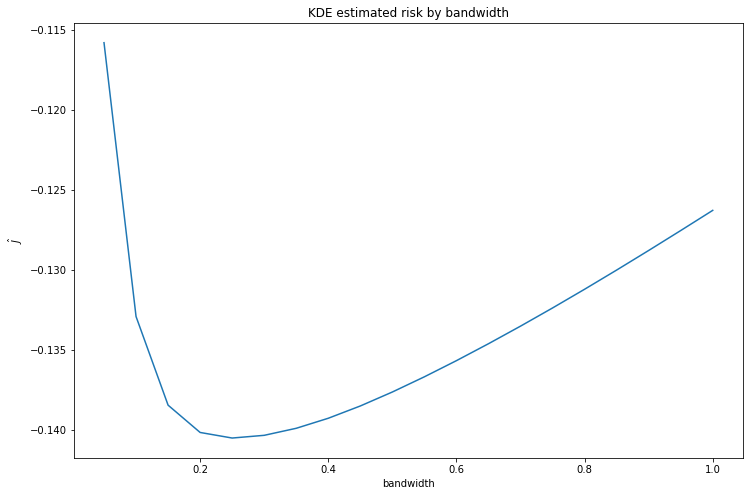
\includegraphics[width=0.9\linewidth,height=0.2\textheight,keepaspectratio]{Figure-21-02}
\end{figure}
    
\begin{console}
Best bandwidth:                 0.252
Risk with selected bandwidth:   -0.141
\end{console}

\begin{python}
def plot_histogram(X, bins, ax):
    X_min, X_max = X.min(), X.max()
    x_plot_vals = np.arange(X_min - 0.05 * (X_max - X_min), X_max + 0.05 * (X_max - X_min), step=(X_max - X_min)/1000)
    
    # Draw the plot
    vals, lower_vals, upper_vals = create_histogram(X, m=bins, alpha=0.05)(x_plot_vals)
    ax.plot(x_plot_vals, vals, color='darkblue', label='Histogram')
    ax.plot(x_plot_vals, upper_vals, color='darkgreen', alpha=0.5, label='95% upper confidence')
    ax.plot(x_plot_vals, lower_vals, color='darkred', alpha=0.5, label='95% lower confidence')
    ax.legend()
    
    # Title and labels
    ax.set_title('bins = %d' % bins)
    ax.set_xlabel('Refractive Index')

    
# Show 4 different bin counts
plt.figure(figsize=(12, 8))
for i, bins in enumerate([5, 15, 25, 50]):
    
    # Set up the plot
    ax = plt.subplot(2, 2, i + 1)
    plot_histogram(X, bins, ax)

plt.tight_layout()
plt.show()

# Best risk
plt.figure(figsize=(14.5, 8))
plot_histogram(X, bins=17, ax=plt.gca())
plt.show()
\end{python}

\begin{figure}[H]
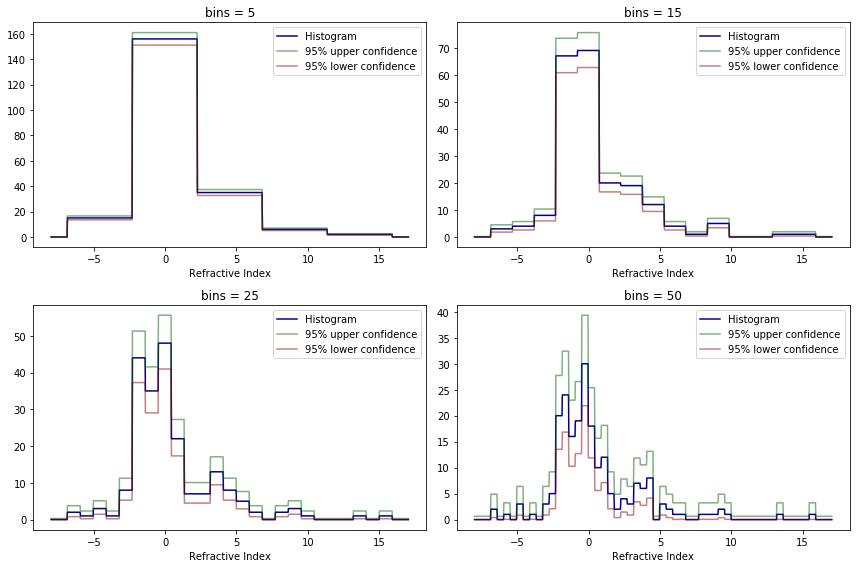
\includegraphics[width=0.9\linewidth,height=0.2\textheight,keepaspectratio]{Figure-21-03}
\end{figure}

\begin{figure}[H]
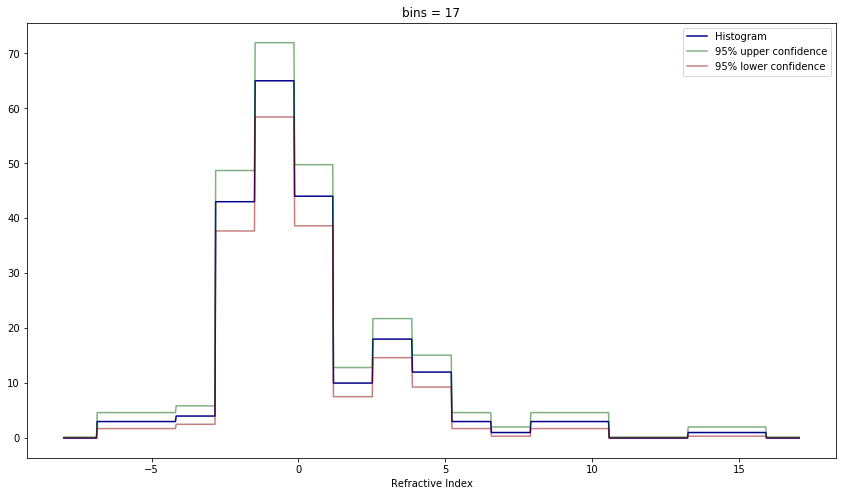
\includegraphics[width=0.9\linewidth,height=0.2\textheight,keepaspectratio]{Figure-21-04}
\end{figure}

\begin{python}
def plot_kde(X, bandwidth, ax):
    X_min, X_max = X.min(), X.max()
    x_plot_vals = np.arange(X_min - 0.05 * (X_max - X_min), X_max + 0.05 * (X_max - X_min), step=(X_max - X_min)/1000)
      
    # Draw the plot
    vals, lower_vals, upper_vals = create_kde(X, bandwidth=bandwidth, alpha=0.05)(x_plot_vals)
    ax.plot(x_plot_vals, vals, color='darkblue', label='KDE')
    ax.plot(x_plot_vals, upper_vals, color='darkgreen', alpha=0.5, label='95% upper confidence')
    ax.plot(x_plot_vals, lower_vals, color='darkred', alpha=0.5, label='95% lower confidence')
    ax.legend()
    
    # Title and labels
    ax.set_title('bandwidth = %.3f' % bandwidth)
    ax.set_xlabel('Refractive Index')    

# Show 4 different bandwidths
plt.figure(figsize=(12, 8))
for i, bandwidth in enumerate([0.05, 0.1, 0.5, 1.0]):
    
    # Set up the plot
    ax = plt.subplot(2, 2, i + 1)
    plot_kde(X, bandwidth, ax)

plt.tight_layout()
plt.show()

# Best risk
plt.figure(figsize=(14.5, 8))
plot_kde(X, bandwidth=best_h, ax=plt.gca())
plt.show()
\end{python}

\begin{figure}[H]
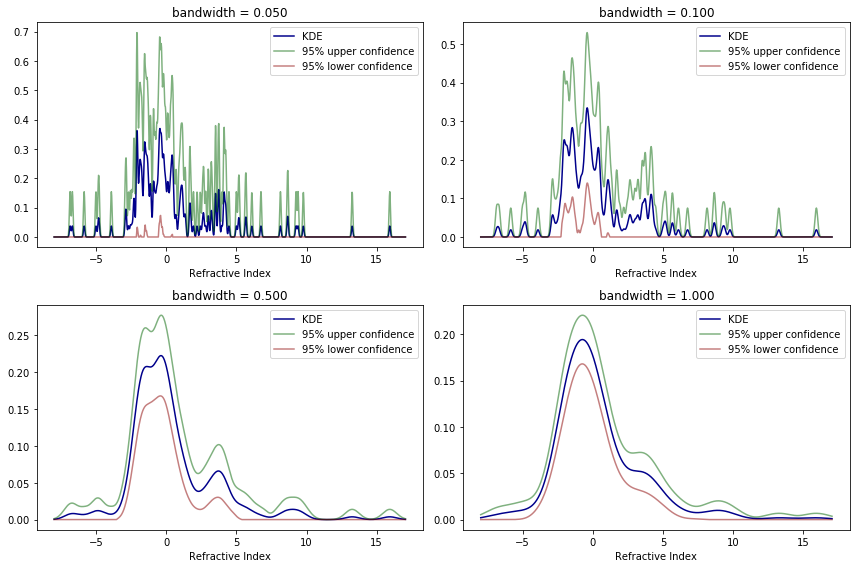
\includegraphics[width=0.9\linewidth,height=0.2\textheight,keepaspectratio]{Figure-21-05}
\end{figure}

\begin{figure}[H]
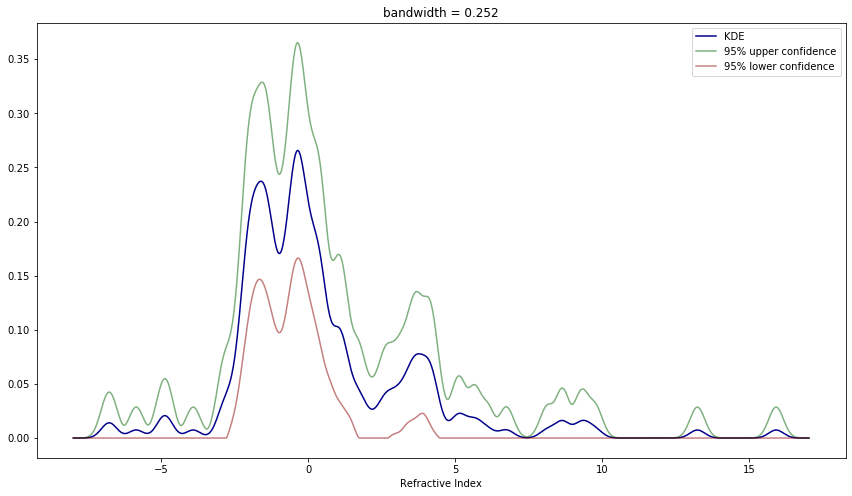
\includegraphics[width=0.9\linewidth,height=0.2\textheight,keepaspectratio]{Figure-21-06}
\end{figure}

In both scenarios the risk estimates helped choose a hyperparameter for
the estimator that produces a convincing and visually pleasing result
for the estimate.

The confidence bands in both examples make it clear that the confidence
bands are around the \textbf{smoothed function} rather than the true
distribution function itself -- there is not a clear relation between
confidence bands for distinct bin sizes, in histograms, or bandwidths,
for KDEs.

\textbf{Exercise 21.7.3}. Consider the data from question 2. Let \(Y\)
be the refractive index and let \(x\) be the aluminium content (the
fourth variable). Do a nonparametric regression to fit the model
\(Y = f(x) + \epsilon\). Use cross-validation to estimate the bandwidth.
Construct 95\% confidence bands for your estimate.

\textbf{Solution}.

\begin{python}
import numpy as np
import pandas as pd

data = pd.read_csv('data/glass.txt', delim_whitespace=True)
X, Y = data['RI'], data['Al']
\end{python}

\begin{python}
import matplotlib.pyplot as plt

plt.figure(figsize=(12, 8))
plt.scatter(X, Y, marker='x')
plt.xlabel('Refractive Index')
plt.ylabel('Al content')
plt.show()
\end{python}

\begin{figure}[H]
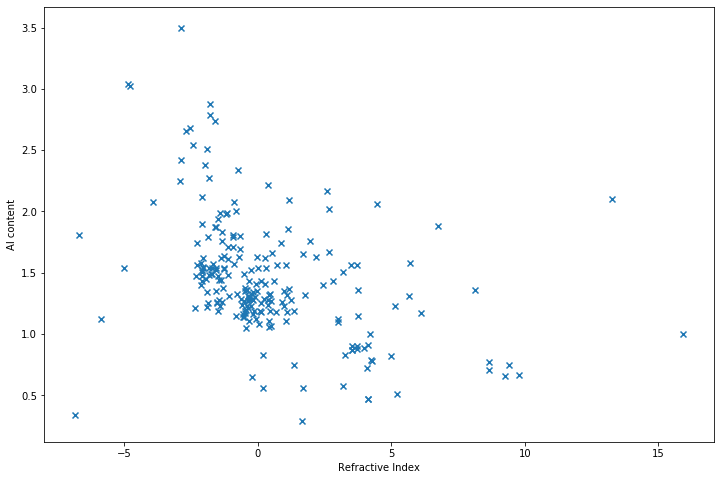
\includegraphics[width=0.9\linewidth,height=0.2\textheight,keepaspectratio]{Figure-21-07}
\end{figure}

The approximate risk when using the Nadaraya-Watson kernel estimator is:

\[ \hat{J}(h) = \sum_{i=1}^n (Y_i - \hat{r}(x_i))^2 \left( 1 - \frac{K(0)}{\sum_{j=1}^n K \left( \frac{x_i - x_j}{h} \right)} \right)^{-2}\]

for a regression given by

\[ \hat{r}(x) = \sum_{i=1}^n w_i(x) Y_i \]

with point weights

\[ w_i(x) = \frac{K\left( \frac{x - x_i}{h} \right)}{\sum_{j=1}^n K\left( \frac{x - x_j}{h} \right)} \]

The confidence bands are computed as with kernel density estimation,
except change the defition of the standard error \(\text{se}(v)\) to

\[ \text{se}(v) = \hat{\sigma} \sqrt{\sum_{i=1}^n w^2_i(v)} \]

where

\[ \hat{\sigma}^2 = \frac{1}{2(n - 1)} \sum_{i=1}^{n-1} (Y_{i+1} - Y_i)^2\]

\begin{python}
def create_nagaraya_watson(X, Y, bandwidth, alpha):
    n = len(X)
    sigma2_hat = np.sum(np.diff(np.sort(Y))**2) / (2 * (n - 1))
    
    def get_values(t):
        XX = np.repeat(X.to_numpy().reshape(-1, 1), len(t), axis=1)
        tt = np.repeat(t.reshape(1, -1), n, axis=0)
        
        # W_ij = w_i(t_j)
        W_unscaled = norm.pdf((tt - XX) / bandwidth) 
        W = W_unscaled / W_unscaled.sum(axis=0)
        
        # R_j = \sum_i W_ji Y_i
        R_j = W.T @ Y
        
        se_V = np.sqrt(sigma2_hat * (W.T**2).sum(axis=1))
        
        Z = norm.pdf((tt - XX) / bandwidth) / bandwidth
        ESS = Z.sum(axis=0) * bandwidth / norm.pdf(0)
        ESS_bar = ESS[np.where(ESS >= 5)].mean()
        q = norm.ppf((1 + (1 - alpha)**(ESS_bar / n)) / 2)
        
        lower = np.maximum(R_j - q * se_V, 0)
        upper = R_j + q * se_V
        
        return R_j, lower, upper
        
    return get_values
\end{python}

\begin{python}
def j_hat_nadaraya_watson(X, Y, h):
    """
    Approximates the risk on a regression using the Nadaraya-Watson kernel estimator:
    
      \hat{J}(h) = \sum_{i=1}^n (Y_i - \hat{r}(x_i))^2 ( 1 - \frac{K(0)}{\sum_{j=1}^n K( \frac{x_i - x_j}{h} )} )^{-2}
      
    where:
      Y_i is the i-th target point
      \hat{r}(x_i) is the estimated regressed value for the i-th point
      K is the regression kernel (assumed to be N(0, 1))
      h is the regression bandwidth
    """
    XX = np.repeat(X.to_numpy().reshape(-1, 1), len(X), axis=1)
    K_values = norm.pdf((XX - X.to_numpy().reshape(1, -1)) / h)
    K_values_sum = K_values.sum(axis=1)
    
    # W_ij = w_i(x_j)
    W = K_values / K_values_sum
    
    # R_j = \sum_i W_ji Y_i 
    R = W.T @ Y
    
    terms = ((Y - R) / (1 - (norm.pdf(0) / K_values_sum)))**2
    
    # Skip NaNs due to zero denominators
    if np.isnan(terms).any():
        return np.nan
    
    return np.sum(terms)
\end{python}

\begin{python}
import matplotlib.pyplot as plt
%matplotlib inline

# Calculate and plot estimated risk for various bandwidths
h_values = np.array([m / 100 for m in range(1, 101)])
j_hat = np.array([j_hat_nadaraya_watson(X, Y, h) for h in h_values])
\end{python}

\begin{python}
# Find bandwidth that minimizes risk
# Using scipy rather than extensive search, since we are looking over a continuous interval

from scipy.optimize import minimize

res = minimize(fun = lambda h: j_hat_nadaraya_watson(X, Y, h), x0 = 0.35, options={'maxiter': 100}, method = 'Nelder-Mead')

best_h = res.x[0]
best_risk = res.fun
\end{python}

\begin{python}
plt.figure(figsize=(12, 8))
plt.plot(h_values[~np.isnan(j_hat)], j_hat[~np.isnan(j_hat)])
plt.xlabel('bandwidth')
plt.ylabel(r'$\hat{J}$')
plt.title('Nagaraya-Watson estimated risk by bandwidth')
plt.show()

print('Best bandwidth:\t\t\t%.3f' % best_h)
print('Risk with selected bandwidth: \t%.3f' % best_risk)
\end{python}

\begin{figure}[H]
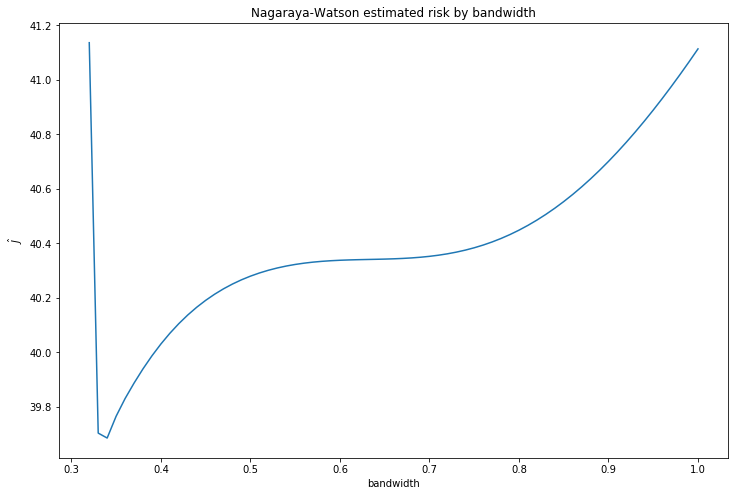
\includegraphics[width=0.9\linewidth,height=0.2\textheight,keepaspectratio]{Figure-21-08}
\end{figure}

\begin{console}
Best bandwidth:                 0.326
Risk with selected bandwidth:   39.204
\end{console}

\begin{python}
def plot_nagaraya_watson(X, Y, bandwidth, ax):
    X_min, X_max = X.min(), X.max()
    x_plot_vals = np.arange(X_min - 0.05 * (X_max - X_min), X_max + 0.05 * (X_max - X_min), step=(X_max - X_min)/1000)
      
    # Draw the plot
    vals, lower_vals, upper_vals = create_nagaraya_watson(X, Y, bandwidth=bandwidth, alpha=0.05)(x_plot_vals)
    ax.scatter(X, Y, color='black', marker='x', alpha=0.2, label='Data')
    ax.plot(x_plot_vals, vals, color='darkblue', label='Regression (Nagaraya-Watson)')
    ax.plot(x_plot_vals, upper_vals, color='darkgreen', alpha=0.5, label='95% upper confidence')
    ax.plot(x_plot_vals, lower_vals, color='darkred', alpha=0.5, label='95% lower confidence')
    ax.legend()
    
    # Title and labels
    ax.set_title('bandwidth = %.3f' % bandwidth)
    ax.set_xlabel('Refractive Index')    
    ax.set_ylabel('Al content')

# Show 4 different bandwidths
plt.figure(figsize=(12, 8))
for i, bandwidth in enumerate([0.05, 0.1, 0.5, 1.0]):
    
    # Set up the plot
    ax = plt.subplot(2, 2, i + 1)
    plot_nagaraya_watson(X, Y, bandwidth, ax)

plt.tight_layout()
plt.show()

# Best risk
plt.figure(figsize=(14.5, 8))
plot_nagaraya_watson(X, Y, bandwidth=best_h, ax=plt.gca())
plt.show()
\end{python}

\begin{figure}[H]
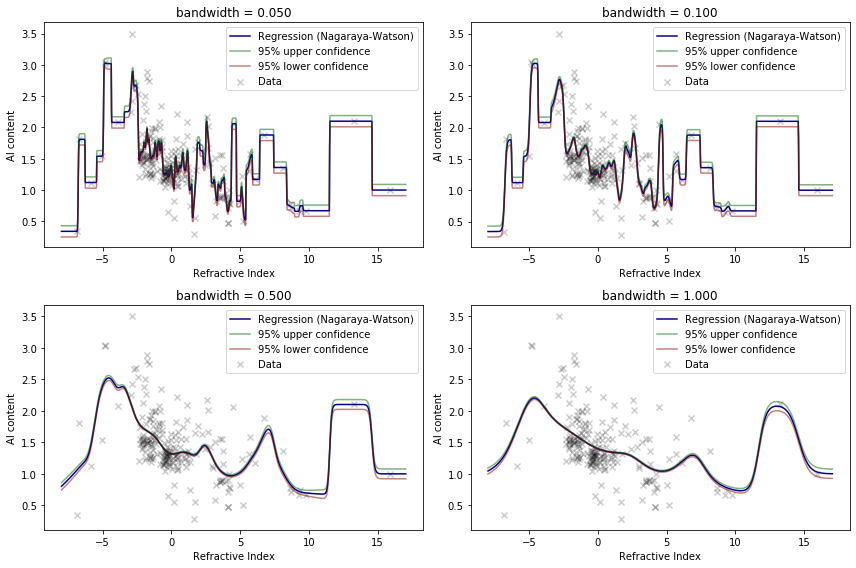
\includegraphics[width=0.9\linewidth,height=0.2\textheight,keepaspectratio]{Figure-21-09}
\end{figure}

\begin{figure}[H]
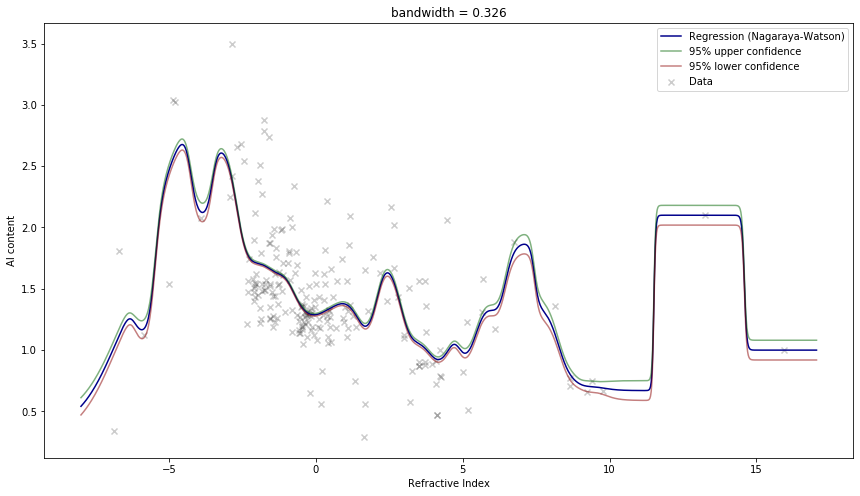
\includegraphics[width=0.9\linewidth,height=0.2\textheight,keepaspectratio]{Figure-21-10}
\end{figure}

\textbf{Exercise 21.7.4}. Prove Lemma 21.1.

The risk can be written as

\[ R(g, \hat{g}) = \int b^2(x) dx + \int v(x) dx \]

where

\[ b(x) = \mathbb{E}(\hat{g}_n(x)) - g(x) \]

is the bias of \(\hat{g}_n(x)\) at a fixed \(x\) and

\[ v(x) = \mathbb{V}(\hat{g}_n(x)) = \mathbb{E}\left( \hat{g}_n(x) - \mathbb{E}(\hat{g}_n(x))^2\right) \]

is the variance of \(\hat{g}_n(x)\) at a fixed \(x\).

\textbf{Solution}.

The risk is defined as

\[ R(g, \hat{g}) = \mathbb{E}\left(L(g, \hat{g}) \right) \]

for the loss function

\[ L(g, \hat{g}) = \int (g(u) - \hat{g}(u))^2 du\]

But we have

\[
\begin{align}
\int b^2(x) dx + \int v(x) dx &= \int (b^2(x) + v(x)) dx \\
&= \int \mathbb{E}(\hat{g}(x) - g(x))^2 + \mathbb{V}(\hat{g}(x)) dx \\
&= \int \mathbb{E}(\hat{g}(x) - g(x))^2 + \mathbb{V}(\hat{g}(x) - g(x)) dx \\
&= \int \mathbb{E}((\hat{g}(x) - g(x))^2) dx \\
&= \mathbb{E}\left(\int (\hat{g}(x) - g(x))^2 dx \right) \\
&= \mathbb{E}(L(g, \hat{g})) \\
&=  R(g, \hat{g})
\end{align}
\]

which proves the lemma.

\textbf{Exercise 21.7.5}. Prove Theorem 21.3.

\[ 
\mathbb{E}(\hat{f}_n(x)) = \frac{p_j}{h} 
\quad \text{and} \quad
\mathbb{V}(\hat{f}_n(x)) = \frac{p_j (1 - p_j)}{nh^2}
\]

for the histogram estimator
\[ \hat{f}_n(x) = \sum_{j=1}^m \frac{\hat{p}_j}{h} I(x \in B_j) \]

\[ \hat{p}_j = \frac{\sum_{i=1}^n I(X_i \in B_j)}{n}
\quad \text{and} \quad
p_j = \int_{B_j} f(u) du \]

\textbf{Solution}.

For \(x \in B_j\), \(\hat{f}_n(x) = \hat{p}_j / h\), since the \(B_j\)
are all disjoint, and only one term of the sum is non-zero. But
\(\hat{p}_j\) is the maximum likelihood estimator for \(p_j\), which is
unbiased, so \(\mathbb{E}(\hat{p}_j) = p_j\) and so

\[\mathbb{E}(\hat{f}_n(x)) = \frac{1}{h} \mathbb{E}(\hat{p}_j) = \frac{p_j}{h}\]

Similarly, \(\mathbb{V}(\hat{f}_n(x)) = \mathbb{V}(\hat{p}_j) / h^2\).
But since
\(n \hat{p}_j = \sum_i I(X_i \in B_j) \sim \text{Binomial}(n, p_j)\),

\[\mathbb{V}(\hat{f}_n(x)) = \frac{1}{h^2} \mathbb{V}(\hat{p}_j) = \frac{1}{n^2h^2} \mathbb{V}\left( \sum_i I(X_i \in B_j) \right) = \frac{1}{n^2h^2} n p_j (1 - p_j) = \frac{p_j (1 - p_j)}{nh^2} \]

\textbf{Exercise 21.7.6}. Prove Theorem 21.7.

\[ \hat{J}(h) = \frac{2}{(n - 1)h} + \frac{n+1}{n-1} \sum_{j=1}^m \hat{p}_j^2 \]

\textbf{Solution}.

We have:

\[ \hat{J}(h) = \int \left( \hat{f}_n(x) \right)^2 dx - \frac{2}{n} \sum_{i=1}^n \hat{f}_{(-i)}(X_i)\]

where \(\hat{f}_{(-i)}\) is the histogram estimator obtained after
removing the \(i\)-th observation.

Let \(v_j\) be the number of samples within the \(j\)-th bin,
\(v_j = \sum_{i=1}^n I(X_i \in B_j)\).

The first term of the cross-validation risk estimator is

\[
\begin{align}
\int \left( \hat{f}_n(x) \right)^2 dx &= \int \left( \sum_{j=1}^m \frac{\hat{p}_j}{h} I(x \in B_j) \right)^2 dx\\
&= \int \left( \frac{1}{nh}  \sum_{j=1}^m \sum_{i=1}^n I(X_i \in B_j) I(x \in B_j) \right)^2 dx \\
&= \frac{1}{n^2h^2} \int \left( \sum_{j=1}^m v_j I(x \in B_j) \right)^2 dx \\
&= \frac{1}{n^2h^2} \left( \int \sum_{j=1}^m v_j^2 I(x \in B_j)^2 dx  + \int \sum_{a, b; a \neq b}  v_a v_b I(x \in B_a) I(x \in B_b) dx\right) \\
&= \frac{1}{n^2h^2} \int \sum_{j=1}^m v_j^2 I(x \in B_j) dx \\
&= \frac{1}{n^2h^2} \sum_{j=1}^m \int_{B_j} v_j^2 dx = \frac{1}{n^2h^2} \sum_{j=1}^m \left| B_j \right| v_j^2 = \frac{1}{n^2h^2} \sum_{j=1}^m h v_j^2 = \frac{1}{n^2h} \sum_{j=1}^m v_j^2
\end{align}
\]

since \(I(s)^2 = I(s)\) and \(B_a, B_b\) are disjoint for \(a \neq b\),
so \(I(x \in B_a) I(x \in B_b) = 0\).

The leave-one-out estimator is:

\[ 
\begin{align}
\hat{f}_{(-i)}(x) &= \sum_{j=1}^m \frac{\hat{p}_{j, (-i)}}{h} I(x \in B_j) \\
&= \sum_{j=1}^m \frac{1}{h} \left( \sum_{k=1, i \neq k}^n \frac{1}{n - 1} I(X_k \in B_j) \right) I(x \in B_j) \\
&= \frac{1}{(n - 1)h} \sum_{j=1}^m \sum_{k=1, i \neq k}^n I(X_k \in B_j) I(x \in B_j)
\end{align}
\]

Then, the sum over the leave-one-out estimators is:

\[
\begin{align}
\sum_{i=1}^n \hat{f}_{(-i)}(X_i) &= \frac{1}{(n - 1)h} \sum_{i=1}^n \sum_{j=1}^m \sum_{k=1, i \neq k}^n I(X_i \in B_j) I(X_k \in B_j) \\
&= \frac{1}{(n - 1)h} \sum_{j=1}^m \sum_{i=1}^n I(X_i \in B_j)\left( \sum_{k=1, i \neq k}^n I(X_k \in B_j) \right)
\end{align}
\]

Note that the inner term \(\sum_{k=1, i \neq k}^n I(X_k \in B_j)\)
counts the number of samples other than \(X_i\) belonging to the bin
\(B_j\), so it is equal to \(v_j - I(X_i \in B_j)\). Replacing that into
the expression,

\[
\begin{align}
\sum_{i=1}^n \hat{f}_{(-i)}(X_i) &= \frac{1}{(n - 1)h} \sum_{j=1}^m \sum_{i=1}^n I(X_i \in B_j) (v_j - I(X_i \in B_j)) \\
&= \frac{1}{(n - 1)h} \sum_{j=1}^m \left( v_j \sum_{i=1}^n I(X_i \in B_j) - \sum_{i=1}^n I(X_i \in B_j)^2 \right) \\
&= \frac{1}{(n - 1)h} \sum_{j=1}^m \left( v_j^2 - v_j \right)
\end{align}
\]

Therefore,

\[
\begin{align}
\hat{J}(h) &= \int \left( \hat{f}_n(x) \right)^2 dx - \frac{2}{n} \sum_{i=1}^n \hat{f}_{(-i)}(X_i) \\
&= \sum_{j=1}^m \left( \frac{1}{n^2h} v_j^2 - \frac{2}{n} \frac{1}{(n - 1)h} \left( v_j^2 - v_j \right) \right)\\
&= \sum_{j=1}^m \left( \frac{(n - 1) v_j^2 - 2n(v_j^2 - v_j)}{n^2(n - 1)h} \right) \\
&= - \frac{n+1}{n^2(n - 1)h} \sum_{j=1}^m v_j^2 + \frac{2n}{n^2(n - 1)h} \sum_{j=1}^m v_j
\end{align}
\]

But we also have that \(\sum_{j=1}^m v_j = n\), since this is a count of
the total number of samples, and that \(v_j = n \hat{p}_j\), so this
expression is equivalent to:

\[ \hat{J}(h) = \frac{2}{(n - 1)h} - \frac{n + 1}{n - 1} \sum_{j=1}^m \hat{p}_j\]

which is the desired result.

\textbf{Exercise 21.7.7}. Prove Theorem 21.14.

For KDE, for any \(h > 0\),

\[ \mathbb{E} \left[ \hat{J}(h) \right] = \mathbb{E} \left[ J(h) \right] \]

Also,

\[ \hat{J}(h) \approx \frac{1}{hn^2}\sum_{i, j} K^* \left( \frac{X_i - X_j}{h} \right) + \frac{2}{nh} K(0) \]

where \(K^*(x) = K^{(2)}(x) - 2 K(x)\) and
\(K^{(2)}(z) = \int K(z - y) K(y) dy\).

\textbf{Solution}. The definitions of \(J(h)\) and \(\hat{J}(h)\) are:

\[ J(h) = \int \hat{f}^2(x) dx - 2 \int \hat{f}(x) f(x) dx 
\quad \text{and} \quad
\hat{J}(h) = \int \hat{f}^2(x) dx - 2 \frac{1}{n} \sum_{i=1}^n \hat{f}_{-i}(X_i) \]

where \(\hat{f}_{-i}\) is the kernel density estimator after omitting
the \(i\)-th observation, and the kernel density estimator is

\[ \hat{f}(x) = \frac{1}{nh} \sum_{i=1}^n K\left( \frac{x - X_i}{h} \right) \]

The leave-one-out estimator is

\[ \hat{f}_{-i}(x) = \frac{1}{(n - 1) h} \sum_{j=1; i \neq j}^n K \left( \frac{x - X_j}{h} \right) \]

We have that

\[ 
\begin{align}
\int \hat{f}(x) f(x) dx &=  \mathbb{E}_x \left[ \mathbb{E}_{X}\left[\hat{f}(x)\right] \right] \\
&= \frac{1}{nh} \sum_{i=1}^n \mathbb{E}_x\left[\mathbb{E}_{X_i}\left[K \left( \frac{x - X_i}{h} \right) \right] \right]  \\
&= \frac{1}{nh} \sum_{i=1}^n \mathbb{E}_x\left[ \int K \left( \frac{x - y}{h} \right) f(y) dy \right] \\
&= \frac{1}{h} \int \int K \left( \frac{x - y}{h} \right) f(x) f(y) dx  dy
\end{align}
\]

and

\[
\begin{align}
\mathbb{E}_X\left[ \hat{f}_{-i}(X_i) \right] &=
\frac{1}{(n - 1) h} \sum_{j=1; i \neq j}^n \mathbb{E}_{X_i}\left[ \mathbb{E}_{X_j}\left[ K \left( \frac{X_i - X_j}{h} \right) \right] \right] \\
&= \frac{1}{(n - 1)} \sum_{j=1; i \neq j}^n \frac{1}{h} \mathbb{E}_{X_i}\left[ \int K \left( \frac{X_i - y}{h} \right) f(y) dy \right] \\
& = \frac{1}{h} \int \int K \left( \frac{x - y}{h} \right) f(x) f(y) dx  dy
\end{align}
\]

so

\[
\begin{align}
\mathbb{E}_X\left[ \int \hat{f}(x) f(x) dx \right] &= \mathbb{E}_X\left[ \frac{1}{n} \sum_{i=1}^n \hat{f}_{-i}(X_i) \right] \\
\mathbb{E}\left[ \int \hat{f}^2(x) dx - 2 \int \hat{f}(x) f(x) dx \right] &= \mathbb{E}\left[ \int \hat{f}^2(x) dx - 2 \frac{1}{n} \sum_{i=1}^n \hat{f}_{-i}(X_i) \right] \\
\mathbb{E}[J(h)] &= \mathbb{E}[\hat{J}(h)]
\end{align}
\]

as desired.

Next, let's look at the expression for the approximation of
\(\hat{J}(h)\).

The first term of the cross-risk validation is

\[ 
\begin{align}
\int \left(\hat{f}(x)\right)^2 dx &= \int \left( \frac{1}{nh} \sum_{i=1}^n K\left( \frac{x - X_i}{h} \right) \right)^2 dx \\
&= \frac{1}{h^2n^2} \int \sum_{i, j} K \left(\frac{x - X_i}{h}\right) K\left(\frac{x - X_j}{h}\right) dx \\
&= \frac{1}{h^2n^2} \sum_{i, j} \int  K \left(\frac{x - X_i}{h}\right) K\left(\frac{x - X_j}{h}\right) dx \\
&= \frac{1}{h^2n^2} \sum_{i, j} \int  K(-y) K\left(-y + \frac{X_i - X_j}{h} \right) h dy \\
&= \frac{1}{hn^2} \sum_{i, j} \int  K\left(\frac{X_i - X_j}{h} - y \right) K(-y) dy \\
&= \frac{1}{hn^2} \sum_{i, j} K^{(2)} \left(\frac{X_i - X_j}{h} \right)
\end{align}
\]

assuming a symmetric kernel, that is, \(K(-y) = K(y)\).

The second term of the cross validation is

\[
\begin{align}
- 2 \frac{1}{n} \sum_{i=1}^n \hat{f}_{-i}(X_i)
&= -2 \frac{1}{n} \sum_{i=1}^n \frac{1}{(n - 1) h} \sum_{j=1; i \neq j}^n K \left( \frac{X_i - X_j}{h} \right) \\
&= -2 \frac{1}{n} \frac{1}{(n - 1) h} \left( \sum_{i, j} K \left( \frac{X_i - X_j}{h} \right) - n K(0)\right) \\
&= \frac{-2}{n (n - 1) h} \sum_{i, j} K \left( \frac{X_i - X_j}{h} \right)
+ \frac{2}{(n - 1) h} K(0) \\
&\approx \frac{-2}{h n^2} \sum_{i, j} K \left( \frac{X_i - X_j}{h} \right)
+ \frac{2}{nh} K(0)
\end{align}
\]

by approximating \(n - 1 \approx n\).

Therefore, the sum of both terms is approximately

\[
\begin{align}
&\frac{1}{hn^2} \sum_{i, j} K^{(2)} \left(\frac{X_i - X_j}{h} \right) + \frac{-2}{h n^2} \sum_{i, j} K \left( \frac{X_i - X_j}{h} \right)
+ \frac{2}{nh} K(0) \\
&= \frac{1}{hn^2} \sum_{i, j} \left( K^{(2)} \left(\frac{X_i - X_j}{h} \right) - 2 K \left( \frac{X_i - X_j}{h} \right) \right) + \frac{2}{nh} K(0) \\
&= \frac{1}{hn^2} \sum_{i, j} K^* \left(\frac{X_i - X_j}{h} \right) + \frac{2}{nh} K(0)
\end{align}
\]

as desired.

\textbf{Exercise 21.7.8}. Consider regression data
\((x_1, Y_1), \dots, (x_n, Y_n)\). Suppose that \(0 \leq x_i \leq 1\)
for all \(i\). Define bins \(B_j\) as in equation 21.7. For
\(x \in B_j\) define

\[ \hat{r}_n(x) = \overline{Y}_j \]

where \(\overline{Y}_j\) is the mean of all the \(Y_i\)'s corresponding
to those \(x_i\)'s in \(B_j\). Find the approximate risk of this
estimator. From this expression for the risk, find the optimal
bandwidth. At what rate does the risk go to zero?

\textbf{Solution}.

The \(m\) bins partition the \([0, 1]\) interval in equal sets as
follows:

\[ B_1 = \left[0, \frac{1}{m} \right), B_2 = \left[\frac{1}{m}, \frac{2}{m} \right), \dots, B_m = \left[\frac{m - 1}{m}, 1 \right] \]

The true regression estimator is

\[ r(x) = \mathbb{E}(Y | X = x) \]

and the risk is the bias squared plus the variance,

\[ R(r, \hat{r}) = \int b^2(x) dx + \int v(x) dx\]

We can now estimate the risk in the same way it was done for the
histogram estimation.

Define a probability distribution function proportional to the true
regression function (shifted to a minimum of 0):

\[ f(x) = \frac{r(x) - r_0}{A} \quad \text{where} \quad A = \int_0^1 r(y) dy - r_0, \quad r_0 = \inf_x r(x) \]

Now, the regression estimator is a scaled up version of the histogram
estimator for \(f\). Therefore,

\[ R(r, \hat{r}) = A^2 R(f, \hat{f}) \]

and we can reuse the results from the histogram estimator in Theorem
21.4.

\[ R(r, \hat{r}) = A^2 R(f, \hat{f}) \approx A^2 \left( \frac{h^2}{12} \int (f'(u))^2 du + \frac{1}{nh} \right) = \frac{h^2}{12} \int (r'(u))^2 du + \frac{A^2}{nh} \]

The value that minimizes it is still

\[ h^* = \frac{1}{n^{1/3}} \left( \frac{6}{\int (f'(u))^2 du} \right)^{1/3} = \frac{1}{n^{1/3}} \left( \frac{6A^2}{\int (r'(u))^2 du} \right)^{1/3}\]

With this choice of bandwidth,

\[ R(r, \hat{r}) = A^2 R(f, \hat{f}) = O(n^{-2/3}) \]

\textbf{Exercise 21.7.9}. Show that with suitable smoothness assumptions
on \(r(x)\), \(\hat{\sigma}^2\) in equation (21.41) is a consistent
estimator of \(\sigma^2\).

\textbf{Solution}. The definition of \(\hat{\sigma}^2\) is

\[ \hat{\sigma}^2 = \frac{1}{2(n - 1)} \sum_{i=1}^{n-1} (Y_{i+1} - Y_i)^2\]

in the context of the Nagaraya-Watson kernel regression estimator, with
sorted \(Y_i\)'s.

The difference between consecutive \(Y_i\)'s is:

\[ Y_{i+1} - Y_i = r(X_{i+1}) - r(X_i) + (\epsilon_{i+1} - \epsilon_i) \approx r'(X_i) (X_{i+1} - X_i) + (\epsilon_{i+1} - \epsilon_i) \]

Assume \(r'(x)\) is finite and bounded, i.e.~\(\sup_x r'(x) < \infty\).

As \(n \rightarrow \infty\), \(X_{i+1} - X_i \rightarrow 0\) while
\(r'(X_i)\) is bounded, so

\[ (Y_{i+1} - Y_i)^2 \rightarrow (\epsilon_{i+1} - \epsilon_i)^2 = \epsilon_{i+1}^2 + \epsilon_i^2 - 2\epsilon_i \epsilon_{i+1} \]

\[ 
\begin{align}
\hat{\sigma}^2 &\rightarrow \frac{1}{2(n - 1)} \left(\sum_{i = 1}^{n - 1} \epsilon_i^2 + \sum_{i = 2}^n \epsilon_i^2 -2 \sum_{i = 1}^{n - 1} \epsilon_i \epsilon_{i+1} \right) \\
&\approx \frac{1}{n - 1} \left( \sum_{i = 1}^{n - 1} \epsilon_i^2 - \sum_{i = 1}^{n - 1} \epsilon_i \epsilon_{i+1} \right) \\
&= \frac{\sigma^2}{n - 1} \left( \sum_{i = 1}^{n - 1} Z_i^2 - \sum_{i = 1}^{n - 1} Z_i Z_{i+1} \right) \\
&= \frac{\sigma^2}{n - 1} \left( \chi_{n - 1}^2 - \sum_{i = 1}^{n - 1} Z_i Z_{i+1} \right)
\end{align}
\]

since the sum of \(n - 1\) squares of independent standard normals has a
\(\chi_{n-1}^2\) distribution, and
\(Z_j = \epsilon_j / \sigma \sim N(0, 1)\).

We have that \(\mathbb{E}(\chi_{n-1}^2) = n - 1\) and
\(\mathbb{E}(Z_i Z_{i+1}) = 0\) since the errors are independent, so
\(\mathbb{E}(\hat{\sigma}^2) \rightarrow \sigma^2\).

Now, let \(\Delta_i = \epsilon_i ( \epsilon_i - \epsilon_{i+1})\). The
expectations of \(\Delta_i\) and \(\Delta_i^2\) are:

\[ \mathbb{E}(\Delta_i) = \mathbb{E}(\epsilon_i^2) - \mathbb{E}(\epsilon_i \epsilon_{i+1}) = \sigma^2 \]

\[ \mathbb{E}(\Delta_i^2) = \mathbb{E}(\epsilon_i^4) -  \mathbb{E}(\epsilon_i^2 \epsilon_{i+1}^2) = \mathbb{E}(\epsilon_i^4) - \mathbb{E}(\epsilon_i^2) \mathbb{E}(\epsilon_{i+1}^2) = 3\sigma^4 - \sigma^4 = 2\sigma^4\]

We can then compute the variance:

\[ \mathbb{V}(\Delta_i) = \mathbb{E}(\Delta_i^2) - \mathbb{E}(\Delta_i)^2 = 2 \sigma^4 - \sigma^4 = \sigma^4 \]

The covariance between distinct, non-adjacent terms
\(\Delta_i, \Delta_j\) where \(|i - j| > 1\) is 0 since the underlying
variables are all drawn from independent variables. The covariance
between consecutive variables \(\Delta_i, \Delta_{i+1}\) is:

\[ \text{Cov}(\Delta_i, \Delta_{i+1}) = \mathbb{E}(\Delta_i \Delta_{i+1}) - \mathbb{E}(\Delta_i) \mathbb{E}(\Delta_{i+1})\]

But

\[ 
\begin{align}
\mathbb{E}(\Delta_i \Delta_{i+1}) &= \mathbb{E}(\epsilon_i \epsilon_{i+1} (\epsilon_i - \epsilon_{i+1}) (\epsilon_{i+1} - \epsilon_{i+2})) \\
&= \mathbb{E}(\epsilon_i \epsilon_{i+1} (\epsilon_i \epsilon_{i+1} - \epsilon_{i+1}^2 - \epsilon_i \epsilon_{i+2} + \epsilon_{i+1} \epsilon_{i+2}) ) \\
&= \mathbb{E}(\epsilon_i^2 \epsilon_{i+1}^2) - \mathbb{E}(\epsilon_i \epsilon_{i+1} \epsilon_{i+2}^2) - \mathbb{E}(\epsilon_i^2 \epsilon_{i+1} \epsilon_{i+2}) + \mathbb{E}(\epsilon_i \epsilon_{i+1}^2 \epsilon_{i+2}) \\
&= \mathbb{E}(\epsilon_i^2) \mathbb{E}(\epsilon_{i+1}^2) - \mathbb{E}(\epsilon_i) \mathbb{E}(\epsilon_{i+1}) \mathbb{E}(\epsilon_{i+2}^2) - \mathbb{E}(\epsilon_i) \mathbb{E}(\epsilon_{i+1}^2) \mathbb{E}(\epsilon_{i+2}) + \mathbb{E}(\epsilon_i) \mathbb{E}(\epsilon_{i+1}^2) \mathbb{E}(\epsilon_{i+2}) \\
&= \mathbb{E}(\epsilon_i^2) \mathbb{E}(\epsilon_{i+1}^2) \\
&= \sigma^4
\end{align}
\]

since all other terms have an odd exponent in one of the \(\epsilon_j\),
and \(\mathbb{E}(\epsilon_j) = 0\). So

\[ \text{Cov}(\Delta_i, \Delta_{i+1}) = \sigma^4 - \sigma^4 = 0\]

The variance of the sum of \(\Delta_i\) is:

\[ \mathbb{V}\left( \sum_{i=1}^{n-1} \Delta_i \right) = \sum_{i=1}^{n-1} \mathbb{V}(\Delta_i) + 2 \sum_{i=1}^{n-2} \text{Cov}(\Delta_i, \Delta_{i+1}) = (n-1) \sigma^4\]

and so

\[ \mathbb{V}(\hat{\sigma}) \rightarrow \frac{1}{(n-1)^2} \mathbb{V}\left( \sum_{i=1}^{n-1} \Delta_i \right) = \frac{1}{n-1} \sigma^4 \]

which goes to 0 as \(n \rightarrow \infty\).

Since \(\mathbb{E}(\hat{\sigma}^2) \rightarrow \sigma^2\) and
\(\mathbb{V}(\hat{\sigma}) \rightarrow 0\), \(\hat{\sigma}^2\) is a
consistent estimator of \(\sigma^2\).
